\documentclass{beamer}							% pro poměr stran 16:9 použijte \documentclass[smaller,aspectratio=169]{beamer}	

\usepackage[upce]{common/beamerthemeUpceFei} 	% základní styly
\usepackage{common/code} 						% formátování zdrojových kódů
\usepackage{common/customs} 					% vlastní příkazy (například obrázek na celou obrazovku)
\usepackage[czech]{babel}						% balíček typografických pravidel jazyka. Můžete využít i "english" místo "czech".

\graphicspath{{images/}} 						% zde jsou umístěny obrázky

\author{Jan Novák}	
\title{Jednoduchá prezentace}
%\institute{Univerzita Pardubice}
%\date{Září 18, 2020} 							%pokud se zakomentuje, vloží se datum posledního uložení

\begin{document}
\maketitle

%%%%%%%%%%%%%%%%%%%%%%%%%%%%%%%%%%%%%%%%%%%%%%%%%%%%%%%%%%%%%%%%%%%%%%%%%%%%
%%%%%%%%%%%%%%%%          ZDE ZAČÍNÁ DOKUMENT       %%%%%%%%%%%%%%%%%%%%%%%%
%%%%%%%%%%%%%%%%%%%%%%%%%%%%%%%%%%%%%%%%%%%%%%%%%%%%%%%%%%%%%%%%%%%%%%%%%%%%


%%%%%%%%%%%%%%%%%%%%%%%%%%%%%%%%%%%%%%%%%%%%%%%%%%%%%%%%%%%%%%%%%%%%%%%%%%%%
\section{Textová sekce}
%%%%%%%%%%%%%%%%%%%%%%%%%%%%%%%%%%%%%%%%%%%%%%%%%%%%%%%%%%%%%%%%%%%%%%%%%%%%
\begin{frame}[fragile, shrink=0]{Seznamy}

	\begin{itemize}
		\item položka
		      \begin{itemize}
			      \item položka
			      \item položka
		      \end{itemize}
		\item položka
		      \begin{itemize}
			      \item položka
		      \end{itemize}
	\end{itemize}
	
		\begin{enumerate}
			\item první řádek
			\begin{itemize}
			      \item položka
			      \item položka
			      \item položka
			      \begin{itemize}
					\item další položka
				
				\end{itemize}
		      \end{itemize}
			\item druhý řádek
			  \begin{enumerate}
			      \item položka
			      \item položka
		      \end{enumerate}
		\end{enumerate}
	
\end{frame}

%%%%%%%%%%%%%%%%%%%%%%%%%%%%%%%%%%%%%%%%%%%%%%%%%%%%%%%%%%%%%%%%%%%%%%%%%%%%
\begin{frame}[fragile, shrink=0]{Matematické výrazy}

\begin{equation}
		< > \subset \supset \subseteq \supseteq \int \sum \prod
\end{equation}

	$$ \alpha, \beta, \gamma, \pi, \Pi, \phi, \varphi, \mu, \Phi $$
	
	$$\lim\limits_{x \to \infty} \exp(-x) = 0$$
	
	$k_{n+1} = n^2 + k_n^2 - k_{n-1}$ 
	
	\begin{math}
	\frac{n!}{k!(n-k)!} = \binom{n}{k}
	\end{math}
	

	$M = \begin{bmatrix}
       \frac{5}{6} & \frac{1}{6} & 0           \\[0.3em]
       \frac{5}{6} & 0           & \frac{1}{6} \\[0.3em]
       0           & \frac{5}{6} & \frac{1}{6}
     \end{bmatrix}$


\begin{itemize}
	\item 	\url{https://oeis.org/wiki/List_of_LaTeX_mathematical_symbols}
\end{itemize}
	
\end{frame}
%%%%%%%%%%%%%%%%%%%%%%%%%%%%%%%%%%%%%%%%%%%%%%%%%%%%%%%%%%%%%%%%%%%%%%%%%%%%
\begin{frame}{Zarovnání položek}
	\begin{itemize}
		\item Odebrat fragile a shrink z definice slajdu
		      \begin{itemize}
			      \item položka
			      \item \textbf{tučně}
		      \end{itemize}
		\item položka
		      \begin{itemize}
			      \item položka
			      \item \emph{kurzíva}
			      \item položka
			      \item \underline{podtržené}
		      \end{itemize}
	\end{itemize}
	
	\cmark   Vytvořit prezentaci 

\xmark   Zaplatit daně 
\end{frame}
%%%%%%%%%%%%%%%%%%%%%%%%%%%%%%%%%%%%%%%%%%%%%%%%%%%%%%%%%%%%%%%%%%%%%%%%%%%%
\begin{frame}{Tabulkový slajd}


\begin{center}
\begin{tabular}{ |l|l|l| }
\hline
\multicolumn{3}{ |c| }{Team sheet} \\
\hline
Goalkeeper & GK & Paul Robinson \\ \hline
\multirow{4}{*}{Defenders} & LB & Lucas Radebe \\
 & DC & Michael Duburry \\
 & DC & Dominic Matteo \\
 & RB & Didier Domi \\ \hline
\multirow{3}{*}{Midfielders} & MC & David Batty \\
 & MC & Eirik Bakke \\
 & MC & Jody Morris \\ \hline
Forward & FW & Jamie McMaster \\ \hline
\multirow{2}{*}{Strikers} & ST & Alan Smith \\
 & ST & Mark Viduka \\
\hline
\end{tabular}
\end{center}


\end{frame}
%%%%%%%%%%%%%%%%%%%%%%%%%%%%%%%%%%%%%%%%%%%%%%%%%%%%%%%%%%%%%%%%%%%%%%%%%%%%
\begin{frame}[fragile, shrink=20]{Dvousloupcový slajd}


\begin{columns}
\begin{column}{0.5\textwidth}
  \begin{itemize}
		\item Položka
		      \begin{itemize}
			      \item položka
			      \item \textbf{tučně}
		      \end{itemize}
	\end{itemize}
   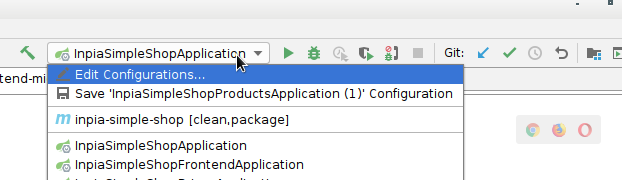
\includegraphics[width=\linewidth]{images/idea-app-configuration.png} 
   
    some text here some text here some text here some text here some text here
\end{column}
\begin{column}{0.5\textwidth}  
    \begin{center}
      \begin{itemize}
		\item Položka
		      \begin{itemize}
			      \item položka
			      \item \textbf{tučně}
		      \end{itemize}
	\end{itemize}
     
     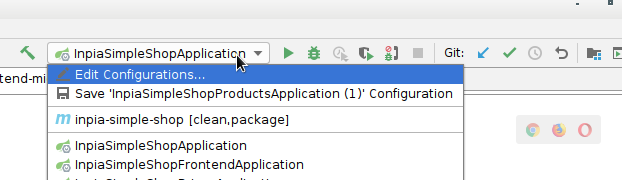
\includegraphics[width=\linewidth]{images/idea-app-configuration.png} 
     
      some text here some text here some text here some text here some text here
     \end{center}
\end{column}
\end{columns}


\end{frame}
%%%%%%%%%%%%%%%%%%%%%%%%%%%%%%%%%%%%%%%%%%%%%%%%%%%%%%%%%%%%%%%%%%%%%%%%%%%%
\section{Obrázková Sekce}
%%%%%%%%%%%%%%%%%%%%%%%%%%%%%%%%%%%%%%%%%%%%%%%%%%%%%%%%%%%%%%%%%%%%%%%%%%%%
\begin{frame}{Běžný slajd I.}
	\begin{itemize}
		\item načítání konfigurace ze vzdáleného serveru
		\item usnadnění nasazení
		\item snadnější správa konfigurací
		\item možnost změny za běhu
		\item konfigurace se může načítat z nejrůznějších zdrojů
		      \begin{itemize}
			      \item GIT, FS, DB
		      \end{itemize}
	\end{itemize}
	\begin{figure}[htp]
		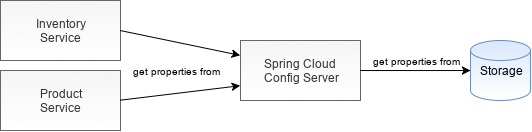
\includegraphics[width=\linewidth]{images/config.png}
	\end{figure}
	\begin{itemize}
		\item \url{http://cloud.spring.io/spring-cloud-config/multi/multi__spring_cloud_config_client.html}
	\end{itemize}
\end{frame}
%%%%%%%%%%%%%%%%%%%%%%%%%%%%%%%%%%%%%%%%%%%%%%%%%%%%%%%%%%%%%%%%%%%%%%%%%%%%
\begin{frame}{Běžný slajd II.}
	\begin{itemize}
		\item bin/startup.sh -- spuštění
		\item conf -- konfigurace
		\item webapps -- místo pro webové aplikace
	\end{itemize}
	\begin{figure}[htp]
		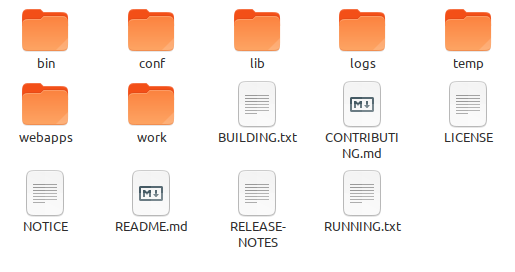
\includegraphics[width=\linewidth]{images/tomcat-webapps.png}
	\end{figure}
\end{frame}
%%%%%%%%%%%%%%%%%%%%%%%%%%%%%%%%%%%%%%%%%%%%%%%%%%%%%%%%%%%%%%%%%%%%%%%%%%%%
\begin{frame}[fragile, shrink=0]{Barvy}
	\begin{itemize}
		\item \textcolor{upce}{UPCE}
		\begin{itemize}
			\item \textcolor{fcht}{FCHT}
			\item \textcolor{fes}{FES}
			\item \textcolor{dfjp}{DFJP}
			\item \textcolor{fei}{FEI}
			\item \textcolor{fzs}{FZS}
			\item \textcolor{ff}{FF} 
			\item \textcolor{fr}{FR} 
		\end{itemize}

		\item Definice barev: \url{http://latexcolor.com/} 
	\end{itemize}
\end{frame}
%%%%%%%%%%%%%%%%%%%%%%%%%%%%%%%%%%%%%%%%%%%%%%%%%%%%%%%%%%%%%%%%%%%%%%%%%%%%
\begin{frame}[fragile, shrink=0]{Obrázkovo-tabulkový slajd}
	\begin{itemize}
		\item v jednom projektu/IDE vytvořit podprojekty
		\item zkusit spustit obě aplikace
		\item zkusit spustit více instancí jedné aplikace

	\end{itemize}

	\begin{tabular}{ll}
		\\
		Konfigurace aplikace                                             & Povolení parallel runu                                                        \\
		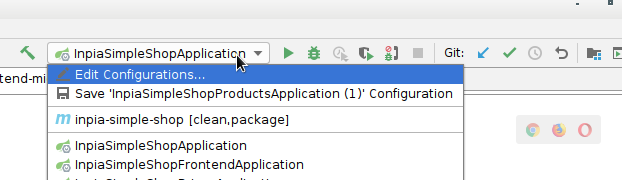
\includegraphics[width=4.5cm]{images/idea-app-configuration.png} & 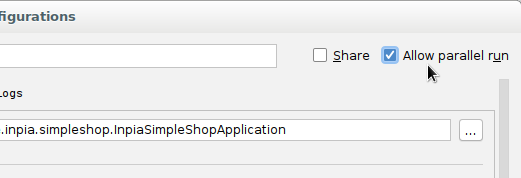
\includegraphics[width=4.5cm]{images/idea-app-configuration-parallel-run.png} \\
		\\
		Struktura projektu                                               & Dashboard                                                                     \\
		
\includegraphics[width=4.5cm]{images/idea-project-structure.png} & 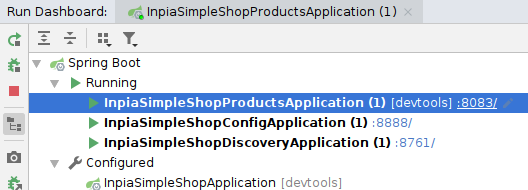
\includegraphics[width=4.5cm]{images/idea-spring-boot-dashboard.png}          \\
	\end{tabular}
\end{frame}
%%%%%%%%%%%%%%%%%%%%%%%%%%%%%%%%%%%%%%%%%%%%%%%%%%%%%%%%%%%%%%%%%%%%%%%%%%%%
\begin{frame}{\zmensi{Slajd s veeeelmi dlouhým nadpisem, který se normálně nevejde na jeden řádek}}
	\begin{itemize}
		\item bin/startup.sh -- spuštění
		\item conf -- konfigurace
		\item webapps -- místo pro webové aplikace
	\end{itemize}

	\begin{figure}[htp]
		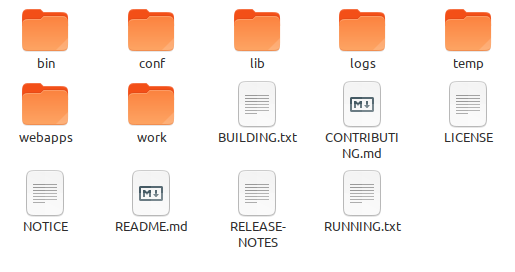
\includegraphics[width=\linewidth]{images/tomcat-webapps.png}
	\end{figure}
\end{frame}
%%%%%%%%%%%%%%%%%%%%%%%%%%%%%%%%%%%%%%%%%%%%%%%%%%%%%%%%%%%%%%%%%%%%%%%%%%%%
\begin{frame}{Obrázek na celou stránku}
	%použít paperwidth nebo paperheight
	\makebox[\linewidth]{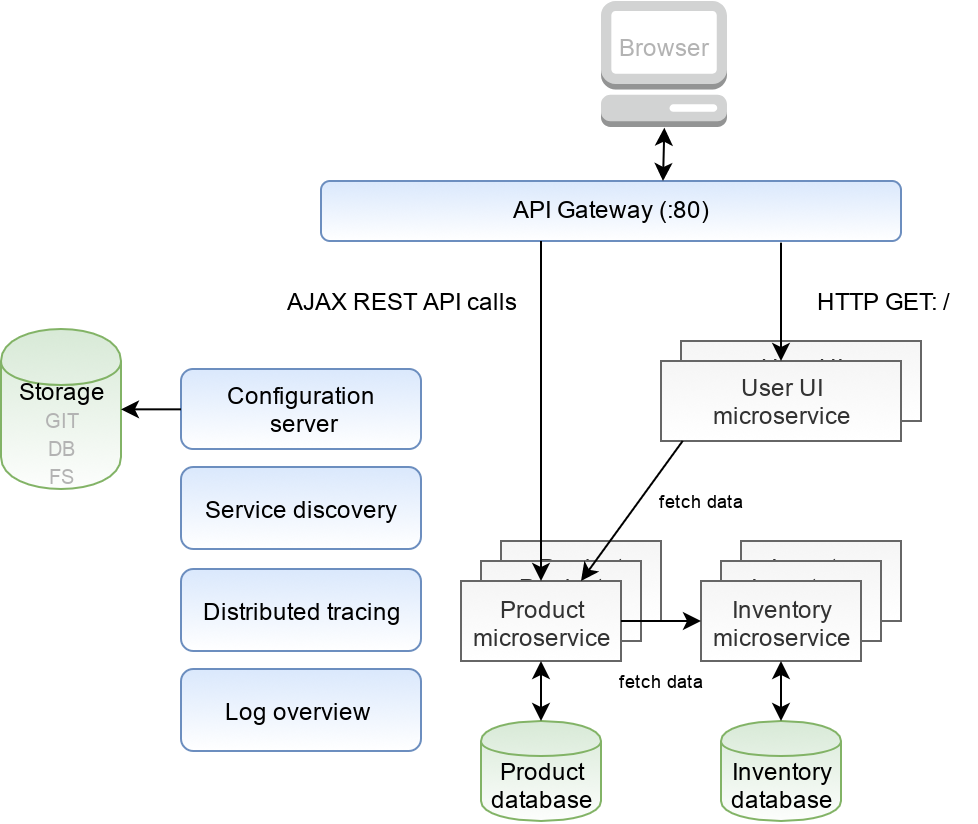
\includegraphics[width=\paperheight]{images/architecture.png}}
\end{frame}
%%%%%%%%%%%%%%%%%%%%%%%%%%%%%%%%%%%%%%%%%%%%%%%%%%%%%%%%%%%%%%%%%%%%%%%%%%%%
\section{Zdrojáková Sekce}
%%%%%%%%%%%%%%%%%%%%%%%%%%%%%%%%%%%%%%%%%%%%%%%%%%%%%%%%%%%%%%%%%%%%%%%%%%%%
\begin{frame}[fragile, shrink=20]{Zdrojové kódy I.}
	PHP
	\begin{lstlisting}[language=PHP]
<?php
// comment
$nums = array(12,2,10,32,23,5);
  sort($nums);
  foreach($nums as $i)
  {
      print($i." = ".var_dump($i)."\n");
  }
  /*commet*/
  $num1 = array('abc'=>10,'abde'=>1,'efg'=>11,'bcd'=>20);
  
  ksort($num1);
  
  print_r($num1);
     
\end{lstlisting}

	Java
	\begin{lstlisting}[language=Java]
@Service
public class ProductServiceImpl implements ProductService {

@Autowired
private ProductClient productClient;

@Override
@HystrixCommand(fallbackMethod = "findAllFallback")
public List<Product> findAll() {
return productClient.findAll();
}

public List<Product> findAllFallback() { ... }
}
\end{lstlisting}
\end{frame}
%%%%%%%%%%%%%%%%%%%%%%%%%%%%%%%%%%%%%%%%%%%%%%%%%%%%%%%%%%%%%%%%%%%%%%%%%%%%
\begin{frame}[fragile, shrink=20]{Zdrojové kódy II.}
	JSON

	\begin{lstlisting}[language=XML]
{ "students": [
      {"id": "1", "name": "Petr"},
      {"id": "2", "name": "Jan"},
      {"id": "3", "name": "Michal"}]
}
\end{lstlisting}

	XML
	\begin{lstlisting}[language=XML]
<dependency>
  <groupId>org.springframework.cloud</groupId>
  <artifactId>spring-cloud-starter-hystrix</artifactId>
</dependency>
\end{lstlisting}
\end{frame}
%%%%%%%%%%%%%%%%%%%%%%%%%%%%%%%%%%%%%%%%%%%%%%%%%%%%%%%%%%%%%%%%%%%%%%%%%%%%
\begin{frame}[fragile, shrink=20]{Zdrojové kódy III.}


	C
	\begin{lstlisting}[language=C]
#include <stdio.h>
int main() {
		int n, reversedNumber = 0, remainder;
		printf("Enter an integer: ");
		scanf("%d", &n);

		while(n != 0)
		{
				remainder = n%10;
				reversedNumber = reversedNumber*10 + remainder;
				n /= 10;
		}
		printf("Reversed Number = %d", reversedNumber);
		return 0;
}
\end{lstlisting}

C++
\begin{lstlisting}[language=C++]
#include <iostream>
using namespace std;
//comment 
int main() {
	int a = 5, b = 10, temp;
	cout << "Before swapping." << endl;
	cout << "a = " << a << ", b = " << b << endl;

	temp = a;
	a = b;
	b = temp;

	cout << "\nAfter swapping." << endl;
	cout << "a = " << a << ", b = " << b << endl;
	return 0;
}
\end{lstlisting}
\end{frame}

%%%%%%%%%%%%%%%%%%%%%%%%%%%%%%%%%%%%%%%%%%%%%%%%%%%%%%%%%%%%%%%%%%%%%%%%%%%%
\begin{frame}[fragile, shrink=20]{Zdrojové kódy IV.}
	R
	\begin{lstlisting}[language=R]
df <- iris[, -5]
summary(df)
df.scaled <- scale(df, center = TRUE, scale = TRUE)
correlation <- cor(df.scaled)
eig <- eigen(correlation)
loadings <- eig$vectors

variance <- eig$values*100/sum(eig$values) # Variances in percentage
cumvar <- cumsum(variance) # Cumulative variances
\end{lstlisting}

	Matlab
	\begin{lstlisting}[language=Matlab]
function max = mymax(n1, n2, n3, n4, n5)

%This function calculates the maximum of the
% five numbers given as input
max =  n1;
if(n2 > max)
	max = n2;
end
if(n3 > max)
	max = n3;
end
if(n4 > max)
	max = n4;
end
if(n5 > max)
	max = n5;
end
\end{lstlisting}
\end{frame}
%%%%%%%%%%%%%%%%%%%%%%%%%%%%%%%%%%%%%%%%%%%%%%%%%%%%%%%%%%%%%%%%%%%%%%%%%%%%
\begin{frame}[fragile, shrink=20]{Zdrojové kódy V.}
	HTML5
	\begin{lstlisting}[language=HTML5]
<!doctype html>
<html lang="en">
<head>
<meta charset="utf-8">
<title>The HTML5 Template</title>
<link rel="stylesheet" href="css/styles.css?v=1.0">
</head>
<body>
Content
<script src="js/scripts.js"></script>
</body>
</html>
\end{lstlisting}

	CSS
	\begin{lstlisting}[language=CSS]
#uniqueId {
width: 100%;
padding: 12px 20px;
margin: 8px 0;
box-sizing: border-box;
}
.className {
border-style: solid;
border-width: 5px;
}
\end{lstlisting}
\end{frame}
%%%%%%%%%%%%%%%%%%%%%%%%%%%%%%%%%%%%%%%%%%%%%%%%%%%%%%%%%%%%%%%%%%%%%%%%%%%%
\begin{frame}[fragile, shrink=20]{Zdrojové kódy VI.}
	JavaScript
	\begin{lstlisting}[language=HTML5]
<!doctype html>
<html lang="en">
<head>
<meta charset="utf-8">
<title>The HTML5 Template</title>
<link rel="stylesheet" href="css/styles.css?v=1.0">
</head>
<body>
Content
<script src="js/scripts.js"></script>
</body>
</html>
\end{lstlisting}

	CSS
	\begin{lstlisting}[language=HTML5]
#uniqueId {
width: 100%;
padding: 12px 20px;
margin: 8px 0;
box-sizing: border-box;
}
.className {
border-style: solid;
border-width: 5px;
}
\end{lstlisting}
\end{frame}
%%%%%%%%%%%%%%%%%%%%%%%%%%%%%%%%%%%%%%%%%%%%%%%%%%%%%%%%%%%%%%%%%%%%%%%%%%%%



\end{document}